\chapter{Enterprise governance and operating models}

\section{Engineering principles}

Governance establishes who may authorize which effects, not merely which prompts are recommended. Separate task sponsor, worker identity, verifier, reviewer, release owner and platform administrator. Classify code and data before enabling external inference or MCP endpoints. Maintain an approved inventory of tools, models, skills and execution images, with review and expiration dates.\src{W1,G3,A10,O5}

\section{Implementation approach}

Define policy-as-code for permitted repositories, paths, destinations and credentials. Require independent review of configuration and skill changes. Establish onboarding, periodic access review, incident response, revocation and rollback procedures. Record task IDs, commit IDs, versions, approval identity and check outcomes. Retain logs only as needed under the applicable data policy. Use risk tiers to keep low-risk changes efficient while requiring escalation for privileged effects.

\section{Verification and limitations}

Audit a sample task from request through release, confirm separation of duties and verify that revoked identities cannot invoke tools. Governance standards must be adapted to applicable legal and organizational obligations; this guide does not certify compliance.

Figure~\ref{fig:d21} illustrates the conceptual flow from Candidate digest to Protected handoff. The edges describe the proposed integration or control relationship, not undocumented internal calls.

\begin{figure}[htbp]\centering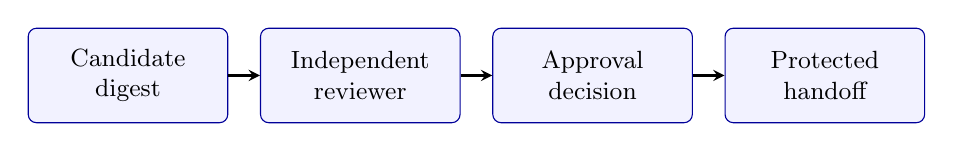
\begin{tikzpicture}[nodebox/.style={draw=blue!60!black,fill=blue!5,rounded corners=3pt,minimum height=12mm,text width=23mm,align=center,font=\small},>=stealth]
\node[nodebox] (n0) at (0.00,0.00) {Candidate digest};
\node[nodebox] (n1) at (2.95,0.00) {Independent reviewer};
\node[nodebox] (n2) at (5.90,0.00) {Approval decision};
\node[nodebox] (n3) at (8.85,0.00) {Protected handoff};
\draw[->,thick] (n0.east) -- (n1.west);
\draw[->,thick] (n1.east) -- (n2.west);
\draw[->,thick] (n2.east) -- (n3.west);
\end{tikzpicture}
\caption{Human approval workflow (conceptual view).}\label{fig:d21}\end{figure}

\section{Chapter conclusion}

Apply the stated verification criteria before expanding the scope of this workflow. Record deviations, evidence and unresolved risks in the task record.
